\documentclass{TDP003mall}
\usepackage{graphicx}
\usepackage{wrapfig}
\graphicspath{{images/}}


\newcommand{\version}{Version 1.1}
\author{Elliot Johansson, \url{elljo130@student.liu.se}\\
  Nadim Lakrouz, \url{nadla777@student.liu.se}}
\title{LoFi-Prototyp}
\date{2022-09-25}
\rhead{Elliot Johansson\\
Nadim Lakrouz}



\begin{document}
\projectpage


\section{Kort beskrivning}

Först befinner man sig på Home page som innehåller navigationsknapparna: Home, Projects och Techniques. Under navigationen finns en kort "about me" stycke. Sen kan man se featured projects som är ett fåtal utvalda project som man vill visa och längst ner på sidan finns en footer med kontaktuppgifter.

Om man väljer att gå till projects sidan lyser projects upp i navigationen och man kommer till sidan där man kan se alla projekt. Under navigationsbaren finns en search bar om man vill leta efter ett specifikt projekt. Man kan även sortera efter tekniker och sök fält där kan man kan välja flera samtidigt. Man kan även välja stigande och fallande träffordning genom att trycka på pilarna vid  SORT BY  där man också kan välja ordningen sökträffar ska sorteras i. Om man klickar in på en projekt så kommer man till
project page där överst på sidan ser en bild av projektet med en beskrivning av det under. Längst ner ser man en lista med techniques som använts i projektet.

Sista sidan man kan ta sig till i navigationen är techniques där man har en tabell av knappar som man kan använda för att filtrera ut projekt efter de tekniker som använts i projektet. Under knapparna finns en lista med alla projekt. Man kan välja flera knappar åt gången och när man trycker på dem så visas de projekt som använt de nedtryckta knapparnas tekniker.

\section{Home}
\begin{center}
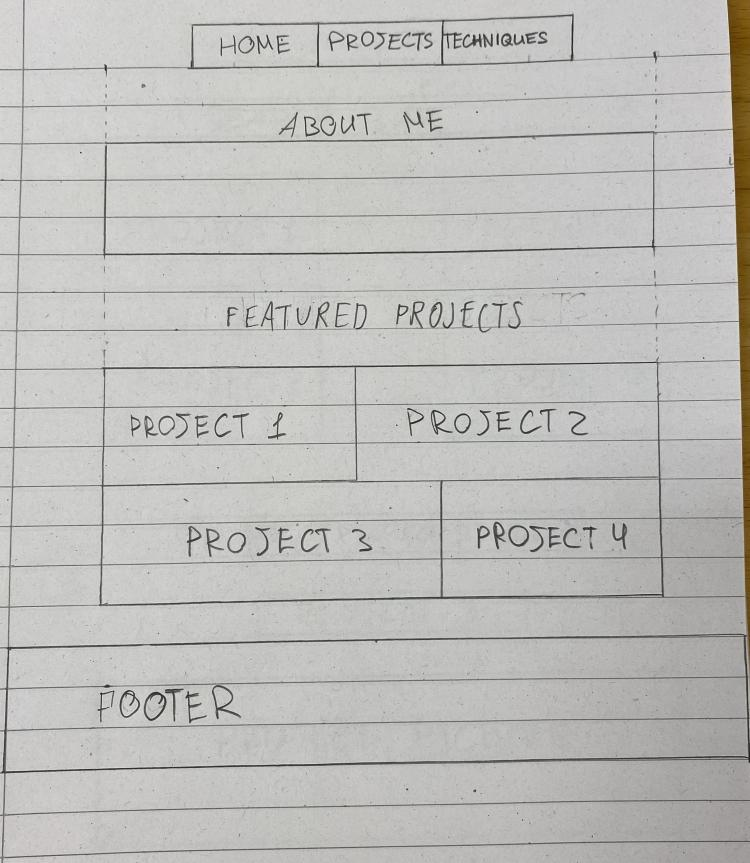
\includegraphics[scale=0.35]{Home.jpg}
\end{center}

\section{Projects}
\begin{center}
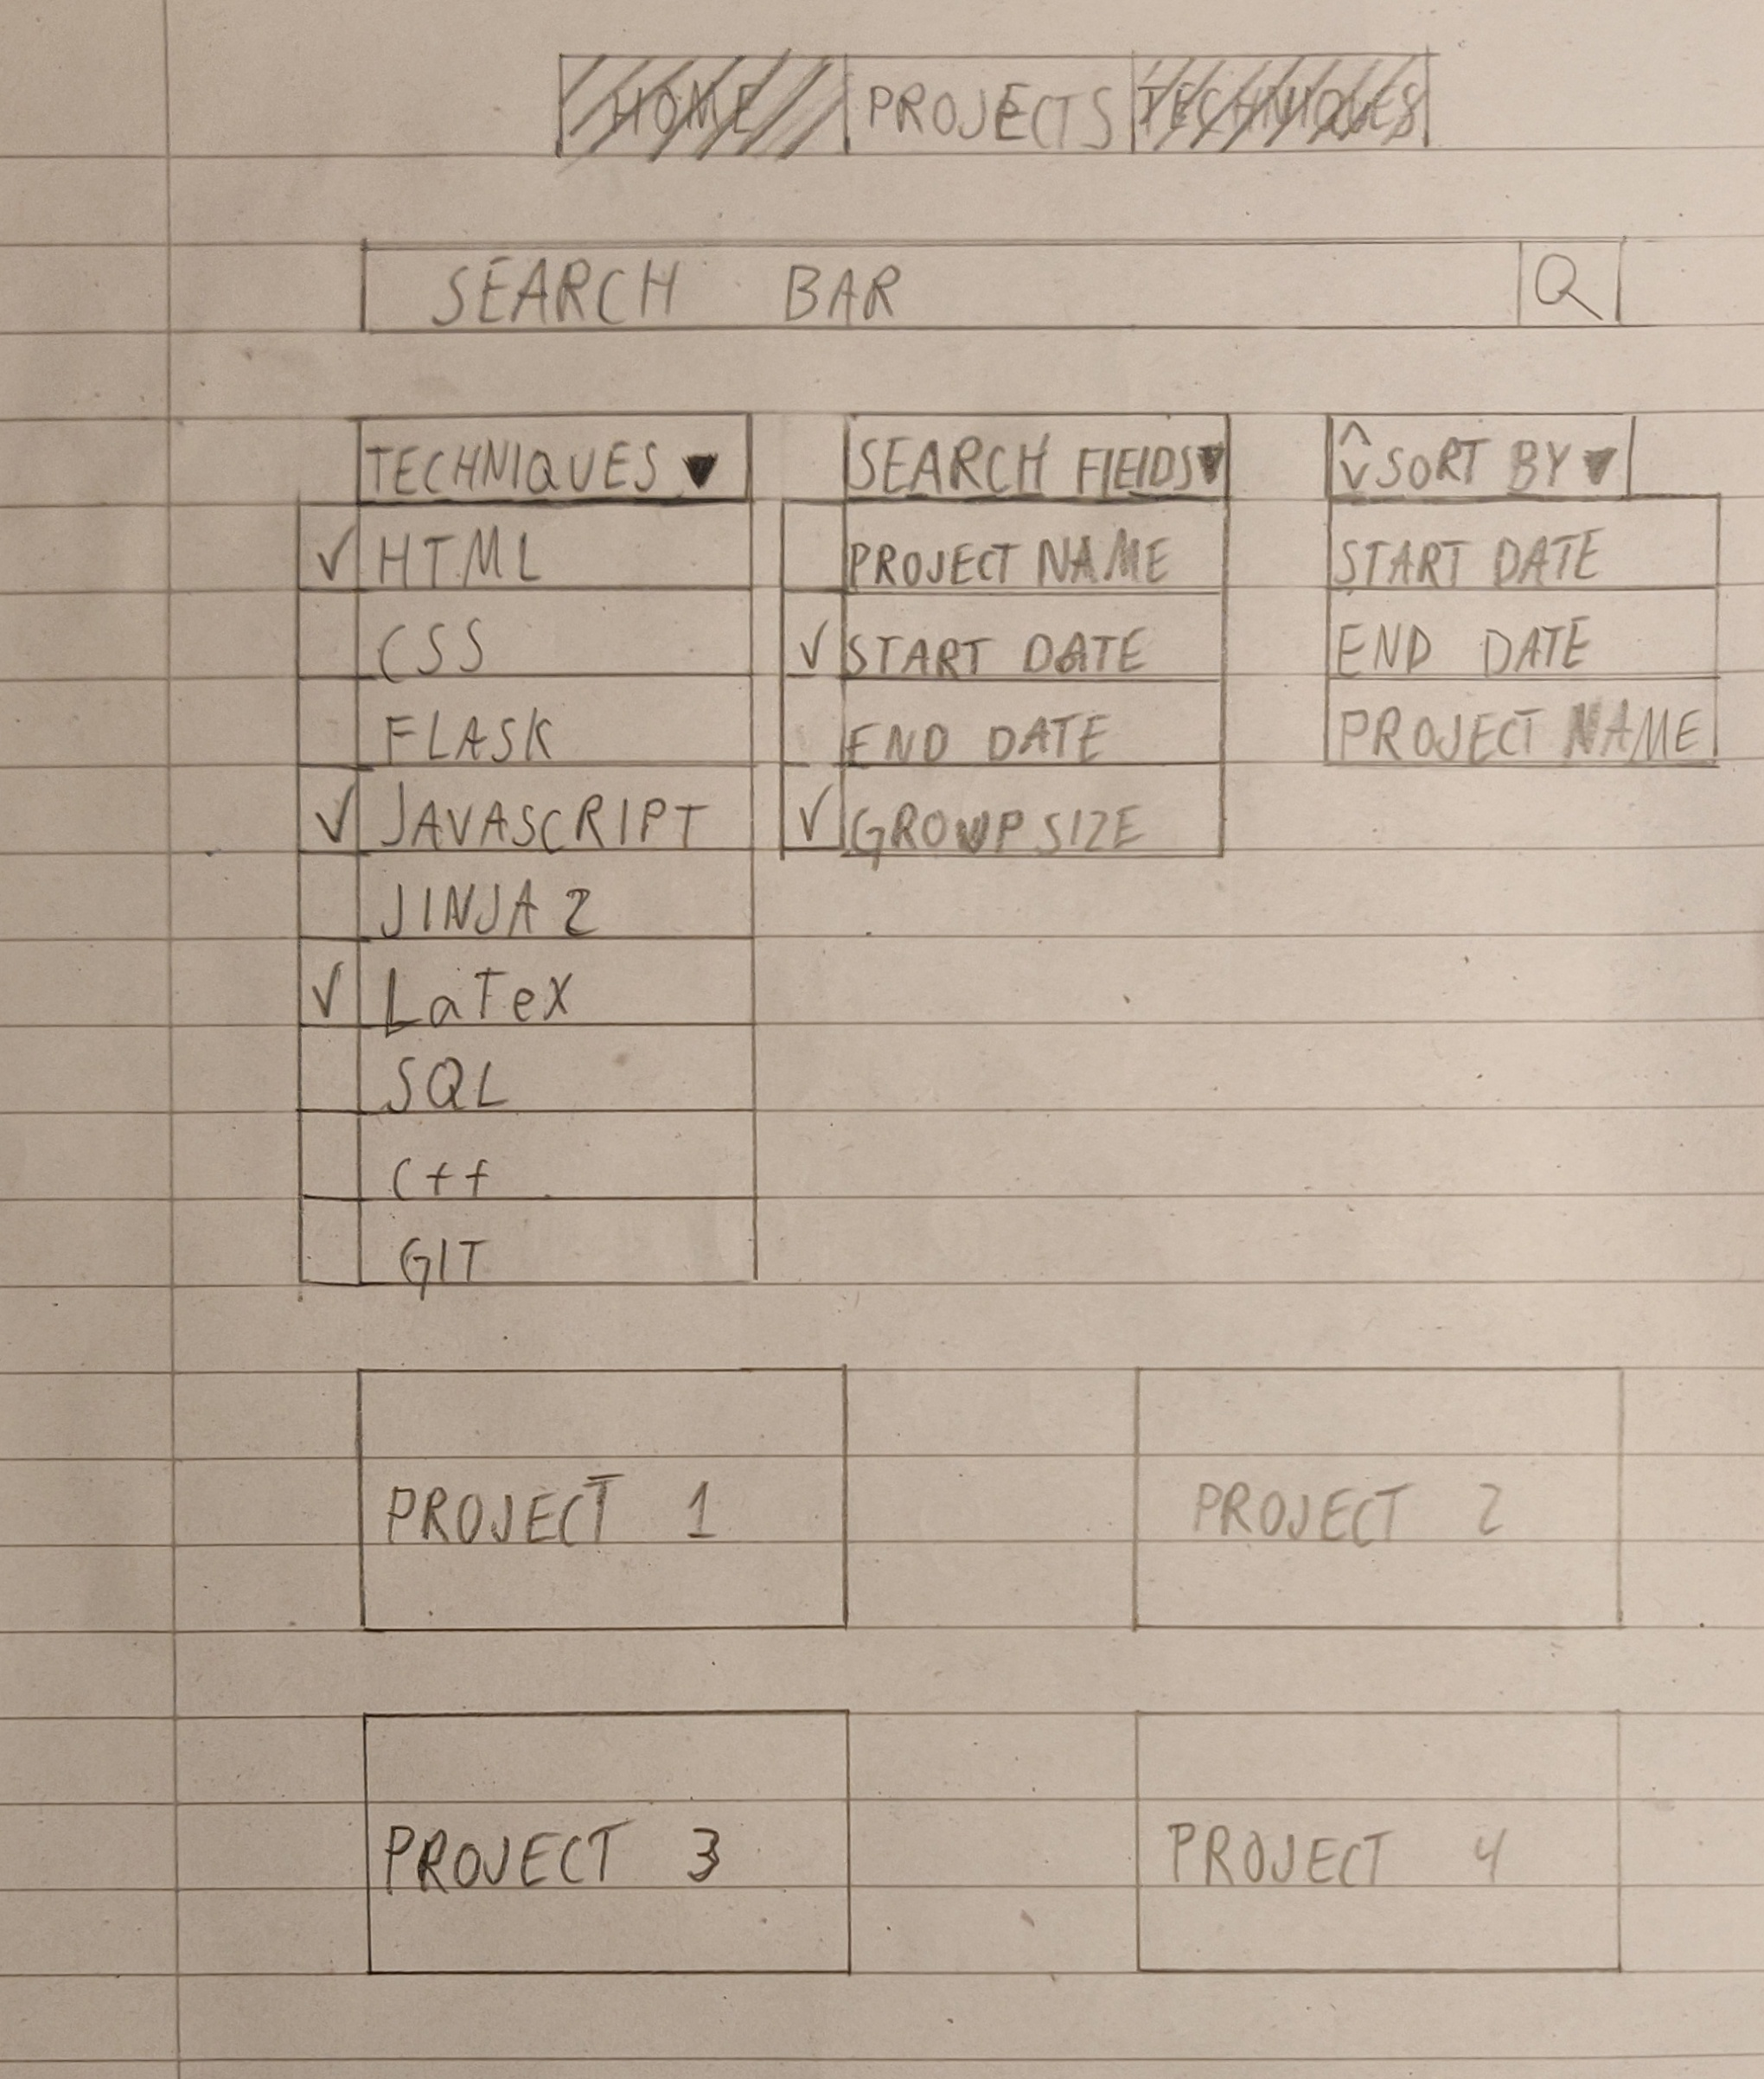
\includegraphics[scale=0.25]{Projects2.jpg}
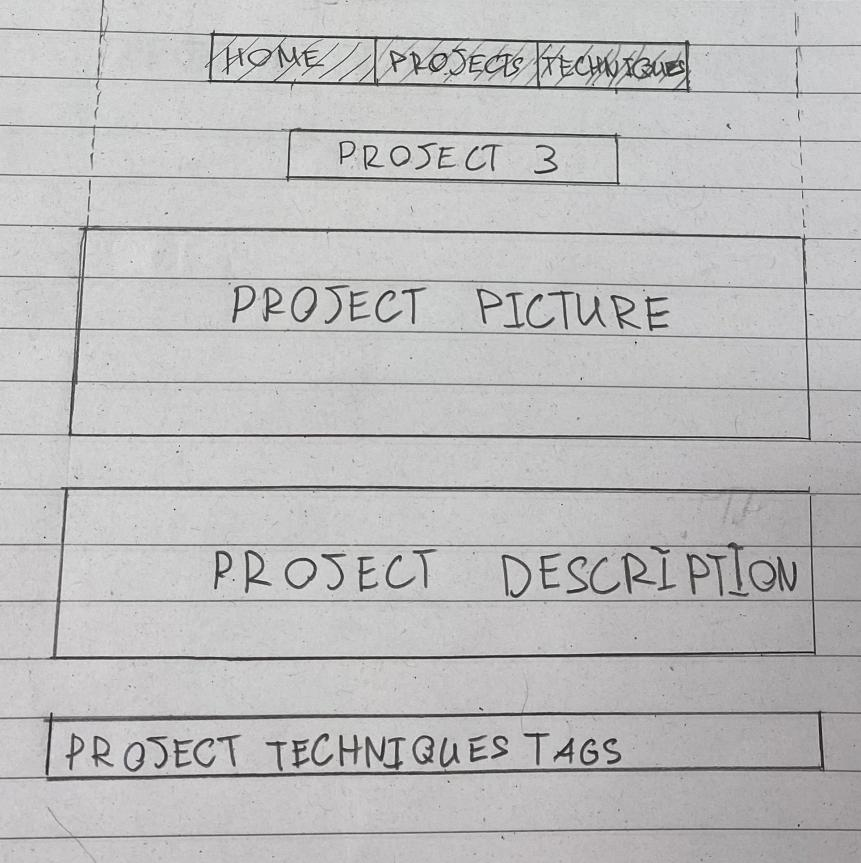
\includegraphics[scale=0.25]{Project.jpg}
\end{center}

\section{Techniques}

\begin{center}
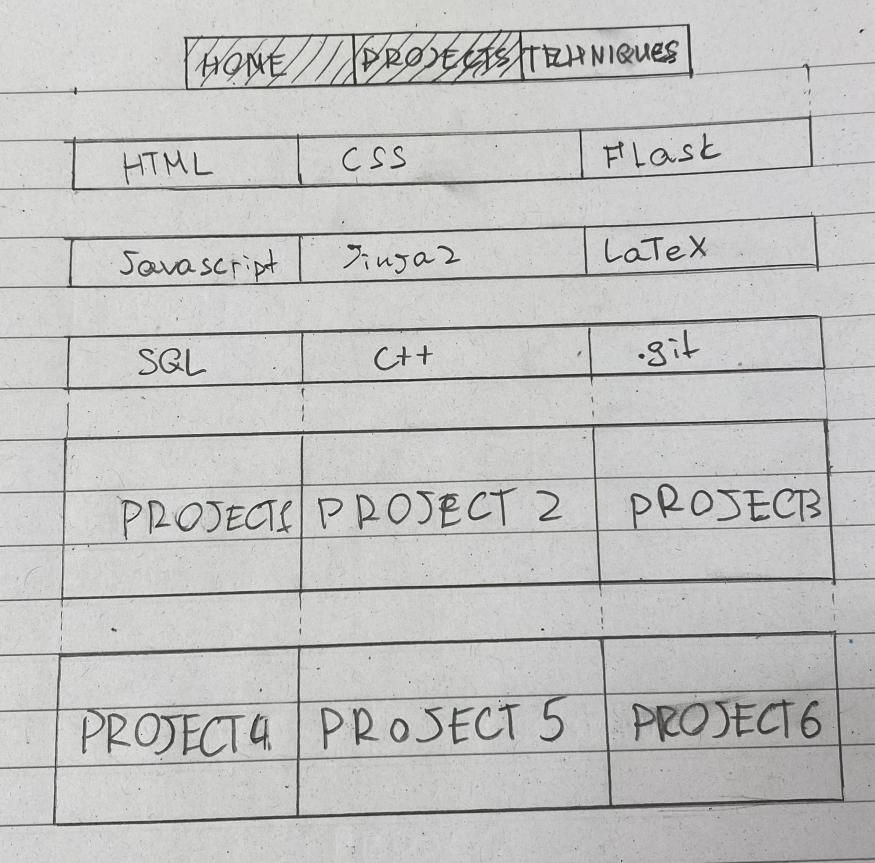
\includegraphics[scale=0.25]{Tech1.jpg}
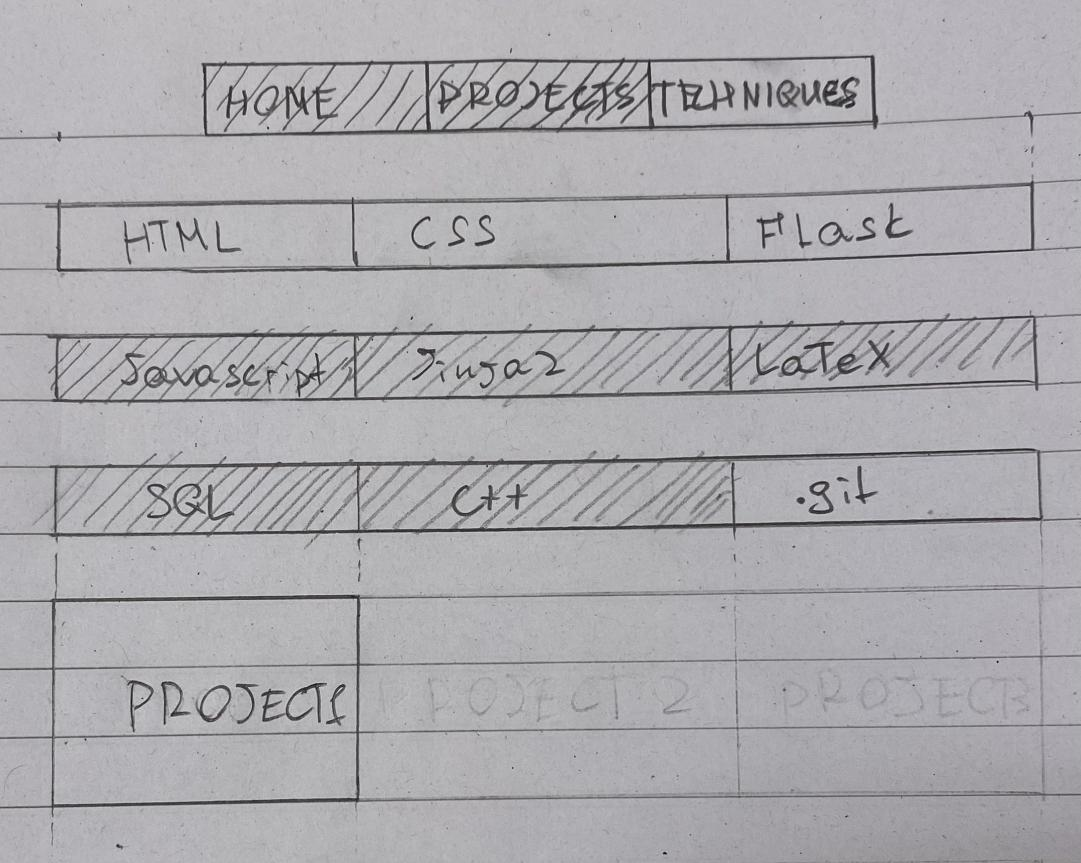
\includegraphics[scale=0.25]{Tech2.jpg}
\end{center}


\end{document}
